%==============================================================================
% Section 9 -- 3DGS for SLAM
%==============================================================================
\section{3D Gaussian Splatting for SLAM}
\label{sec:slam}

\subsection{Simultaneous Localisation and Mapping}

Simultaneous Localisation and Mapping (SLAM) addresses the chicken-and-egg
problem of robotic perception: a moving agent must estimate its own pose
(localisation) while concurrently building a map of the environment (mapping),
without prior knowledge of either.  Classical SLAM pipelines rely on sparse or
semi-dense geometric representations such as point clouds, occupancy grids, and
keyframe-based pose graphs.  These representations are efficient but lack visual
fidelity, making them unsuitable for applications that require photorealistic
reconstructions, such as augmented reality or human-robot interaction.

3DGS offers a compelling alternative: the same Gaussian primitives used for
novel-view synthesis can serve as the scene map, providing simultaneously a
dense, photorealistic, and differentiable representation that can be queried or
rendered in real time.

%------------------------------------------------------------------------------
\subsection{Integration of 3DGS into the SLAM Pipeline}

A 3DGS-SLAM system alternates between two tightly coupled phases:

\begin{enumerate}
  \item \textbf{Tracking.}  Given the current Gaussian map, the camera pose
        $T_t \in SE(3)$ is estimated by minimising a photometric loss between
        the rendered frame (obtained by splatting the existing Gaussians from
        the candidate pose) and the actual camera observation:
        \begin{equation}
          T_t^* = \arg\min_{T_t} \sum_{p} \bigl\|
            \hat{I}(p;\,T_t,\,\mathcal{G}) - I_t(p)
          \bigr\|_1,
          \label{eq:slam_tracking}
        \end{equation}
        where $\hat{I}(p;\,T_t,\,\mathcal{G})$ is the rendered colour at pixel
        $p$ given map $\mathcal{G}$ and pose $T_t$, and $I_t$ is the observed
        frame.

  \item \textbf{Mapping.}  Once the pose is fixed, the Gaussian map is updated
        by (a) spawning new Gaussians at the depth of pixels with high
        photometric error, and (b) optimising all Gaussian parameters via
        back-propagation through the differentiable renderer, exactly as in
        the offline 3DGS pipeline (Section~\ref{sec:optimization}).
\end{enumerate}

\begin{figure}[H]
  \centering
  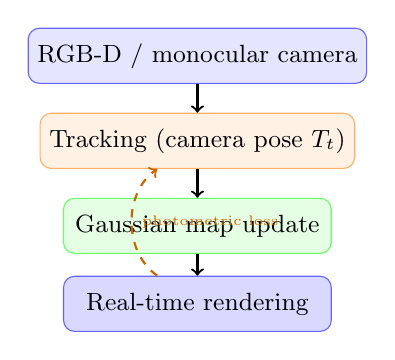
\begin{tikzpicture}[scale=0.9, every node/.style={font=\small},
      box/.style={draw, rounded corners, minimum width=3.4cm,
                  minimum height=0.7cm, align=center}]
    \node[box, fill=blue!10,   draw=blue!60]   (cam)   at (0,3.5) {RGB-D / monocular camera};
    \node[box, fill=orange!10, draw=orange!60] (track) at (0,2.3) {Tracking (camera pose $T_t$)};
    \node[box, fill=green!10,  draw=green!60]  (map)   at (0,1.1) {Gaussian map update};
    \node[box, fill=blue!15,   draw=blue!60]   (ren)   at (0,0.0) {Real-time rendering};
    \draw[->, thick] (cam)   -- (track);
    \draw[->, thick] (track) -- (map);
    \draw[->, thick] (map)   -- (ren);
    \draw[->, thick, dashed, orange!80!black] (ren)
      to[bend left=55] node[right, font=\tiny] {photometric loss}  (track);
  \end{tikzpicture}
  \caption{Data-flow in a 3DGS-SLAM system.  Tracking and mapping alternate
           at each keyframe; the differentiable renderer couples both phases.}
  \label{fig:slam_pipeline}
\end{figure}

%------------------------------------------------------------------------------
\subsection{Notable 3DGS-SLAM Systems}

\begin{table}[H]
  \centering
  \caption{Comparison of published 3DGS-SLAM methods.}
  \label{tab:slam_systems}
  \renewcommand{\arraystretch}{1.4}
  \begin{tabular}{l p{3.2cm} p{4.0cm} p{3.5cm}}
    \toprule
    \textbf{System} & \textbf{Input} & \textbf{Key contribution} & \textbf{Speed} \\
    \midrule
    SplaTAM~\cite{keetha2024splatam} &
      RGB-D &
      Silhouette-guided densification; first real-time 3DGS SLAM &
      $\sim$10 fps mapping \\
    Gaussian-SLAM &
      RGB-D &
      Online reconstruction with sub-map merging &
      $>$10 fps on one GPU \\
    MonoGaussian &
      Monocular RGB &
      Depth estimated from monocular cues; no depth sensor &
      Real-time capable \\
    \bottomrule
  \end{tabular}
\end{table}

%------------------------------------------------------------------------------
\subsection{Advantages and Open Challenges}

\paragraph{Advantages over classical SLAM representations.}
\begin{itemize}
  \item \textbf{Photorealism.}  The Gaussian map supports novel-view rendering,
        enabling downstream tasks such as loop closure via appearance-based
        place recognition.
  \item \textbf{Differentiability.}  Pose optimisation is formulated as gradient
        descent through the renderer (Eq.~\ref{eq:slam_tracking}), without
        requiring hand-crafted feature descriptors.
  \item \textbf{Real-time rendering.}  The GPU-rasterised pipeline delivers
        $>$90 fps renders even during online mapping.
\end{itemize}

\paragraph{Open challenges.}
\begin{itemize}
  \item \textbf{Memory growth.}  The number of Gaussians grows with scene size,
        making large-scale outdoor SLAM memory-intensive.
  \item \textbf{Loop closure.}  Correcting accumulated drift requires updating
        potentially millions of Gaussians consistently.
  \item \textbf{Dynamic objects.}  Moving people or vehicles violate the static
        scene assumption and produce rendering artefacts.
  \item \textbf{Monocular scale ambiguity.}  Without depth, metric scale must
        be recovered from additional cues or a known object.
\end{itemize}

\begin{keybox}{Summary}
  3DGS-SLAM unifies photorealistic scene reconstruction and real-time
  camera tracking in a single differentiable framework, combining the
  speed of GPU rasterisation with the accuracy of gradient-based pose
  optimisation.  Current systems achieve real-time performance on RGB-D
  input; extending them to monocular and large-scale outdoor settings
  remains an active research area.
\end{keybox}
